% !TeX root = ./main.tex

\chapter{ОБЗОР ТЕХНОЛОГИЙ МОДЕЛИРОВАНИЯ НА ГРАФАХ}

\section{Основные понятия, категории и эволюция графовых технологий анализа пространственных полей}

В теории информационных систем и компьютерного анализа изображений графовое представление служит универсальным связующим звеном между регулярными пиксельными матрицами камер и нерегулярными адаптивными сетками вычислительной физики~[\ref{itm:ablyameyko}, с.~34;~\ref{itm:nedzvedz2012}, с.~19]. Наблюдаемый двумерный биологический или физический объект занимает ограниченную выпуклую область $\Omega=(0,1)^2\subset\Real^2$ единичной площади $|\Omega|=1$. Дискретная регистрация состояния поля в момент времени $t$ порождает взвешенный геометрический граф $G=(V,E,m)$, узлы которого $V=\{1,\dots,N\}$ вложены в пространственные координаты центров пикселей или датчиков $\{x_i\}_{i=1}^N\subset\overline{\Omega}$, рёбра $E$ задают отношение пространственной смежности, а положительные веса $m=(m_1,\dots,m_N)^\top$ определяют площади элементарных ячеек разбиения области с условием сохранения полной меры $\sum_{i=1}^N m_i = |\Omega|=1$~[\ref{itm:eymard}, с.~720].

Для строгого сопоставления полей, рассчитанных на графах различной мощности $N_1\neq N_2$ и различной топологии, в информационных конвейерах многомасштабного анализа вводятся оператор узлового сноса $I_h: C(\overline{\Omega})\to\Real^N$, $(I_h u)_i = u(x_i)$, и оператор пространственного подъёма (продолжения) $P_G: \Real^N\to L^2(\Omega)$, отображающий дискретный вектор узловых значений в непрерывное или кусочно-постоянное поле на единой области $\Omega$. На рисунке~\ref{fig:mesh_gallery} сопоставлены четыре основных класса пространственных графовых дискретизаций одного и того же двухкомпонентного поля интенсивности, охватывающие типовые режимы цифровой микроскопии и сенсорного мониторинга.

\begin{figure}[htbp]
    \centering
    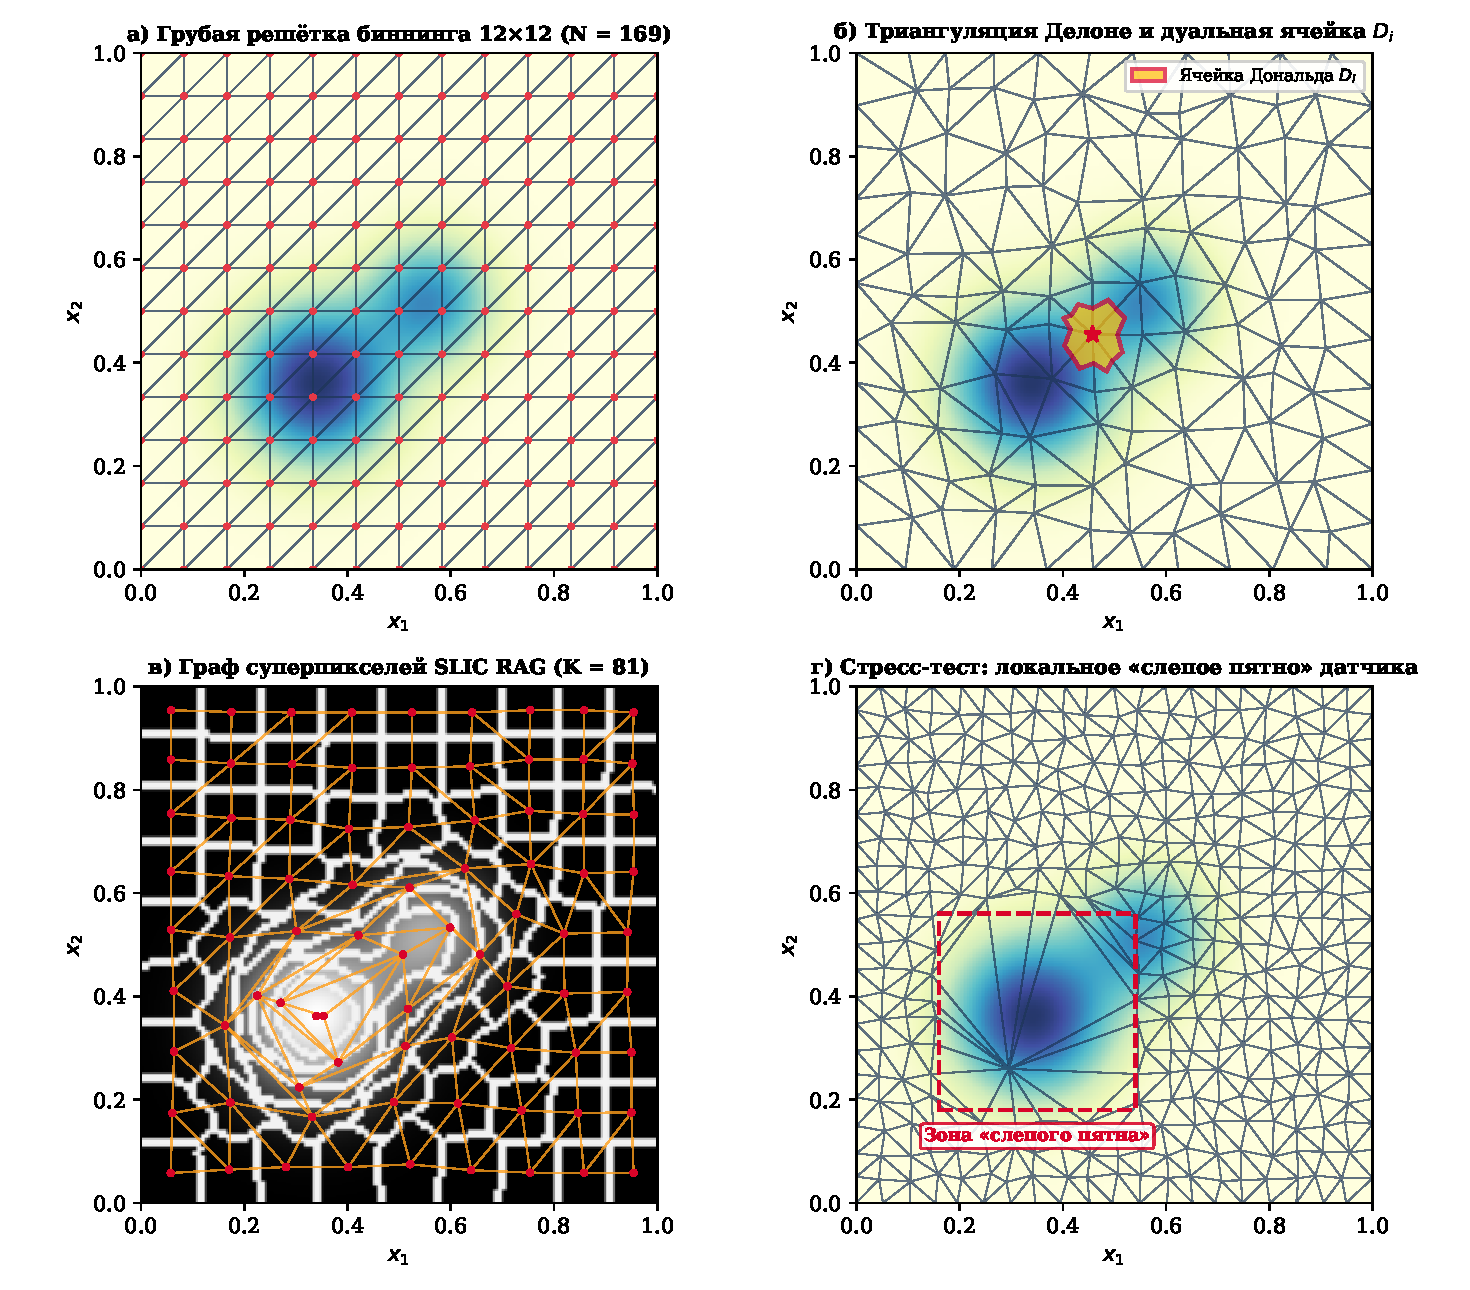
\includegraphics[width=0.80\textwidth]{figures/fig2_mesh_gallery.pdf}
    \caption{Четыре типа пространственных графовых дискретизаций единой области $\Omega=(0,1)^2$: а)~регулярная решётка биннинга; б)~нерегулярная триангуляция Делоне с выделенной барицентрической ячейкой Дональда $D_i$; в)~несимплициальный граф суперпикселей SLIC; г)~сетка с локальным «слепым пятном» датчика}
    \label{fig:mesh_gallery}
\end{figure}

Указанные четыре класса принципиально различаются по своим метрическим и вариационным свойствам:
\begin{itemize}
    \item \emph{регулярные декартовы решётки аппаратного биннинга} формируются при блочном усреднении матрицы детектора ($4\times 4$, $6\times 6$) и характеризуются постоянным шагом $h_G$, но низким пространственным разрешением фронтов;
    \item \emph{конформные симплициальные триангуляции Делоне} адаптируют плотность узлов к геометрии объекта и допускают двойственное разбиение на непересекающиеся барицентрические ячейки Дональда $D_i$ с кусочно-линейным подъёмом $P_G u_G \in H^1(\Omega)$~[\ref{itm:baba}, с.~6];
    \item \emph{несимплициальные графы смежности суперпикселей} (\emph{Region Adjacency Graphs}, SLIC RAG)~[\ref{itm:skimage}] агрегируют однородные по яркости пиксели в многоугольные кластеры со ступенчатыми растровыми границами, нарушающими ортогональность между рёбрами графа и дуальными гранями;
    \item \emph{вырожденные сенсорные сетки с локальными пропусками} («слепыми пятнами») возникают при оптическом насыщении фотоприёмника, артефактах окклюзии или локальном отказе узлов сенсорной сети.
\end{itemize}

Эволюция информационных технологий моделирования динамики на подобных графовых структурах прошла три закономерных историко-методологических этапа:
\begin{enumerate}
    \item \emph{Классические сеточные пакеты метода конечных элементов (МКЭ) и метода конечных объёмов (МКО)}~[\ref{itm:samarsky}, с.~112;~\ref{itm:eymard}] обеспечивают строгую сходимость численного решения при $h_G\to 0$ и точное выполнение дискретных законов сохранения массы, но требуют полного априорного задания тензоров среды и граничных режимов, вследствие чего не предназначены для автоматической идентификации неизвестных параметров переноса по зашумлённым видеопоследовательностям.
    \item \emph{Комбинаторные графовые нейронные сети передачи сообщений (MPNN, GAT) и графовые нейронные ОДУ (GNDE)}~[\ref{itm:gasnikov}, с.~74;~\ref{itm:grand}], активно развивавшиеся в 2016--2022~гг., позволяют обучать векторное поле эволюции непосредственно по данным на фиксированном графе, однако опираются на чисто топологическую матрицу смежности и нормировку по степеням вершин без учёта физических площадей ячеек $m_i$, длин рёбер и ориентации нормалей дуальных граней.
    \item \emph{Инвариантные к дискретизации нейронные операторы и технологии доверительного научного ИИ (2023--2026~гг.)}~[\ref{itm:angelopoulos},~\ref{itm:calvello},~\ref{itm:chin}] формулируют задачу обучения компактного физически интерпретируемого закона на дешёвых грубых сетках с последующим переносом без дообучения (\emph{zero-shot super-resolution transfer}) на произвольные допустимые триангуляции и обязательной выдачей статистически гарантированного интервала погрешности.
\end{enumerate}

\section{Критический анализ подходов к переносимости графовых моделей и сертификации неопределённости}

Систематический анализ профильных публикаций 2020--2026~гг. выделяет четыре конкурирующих теоретических направления в задаче межуровневого переноса графовых моделей и позволяет точно локализовать открытый научно-технологический разрыв:
\begin{enumerate}
    \item \textbf{Спектральная теория переносимости.} В основополагающей работе Р.~Леви, М.~Бронштейна и соавт.~[\ref{itm:levie}, с.~12--18] графовые свёртки трактуются как непрерывные функциональные фильтры $g(\Delta_G)$ самосопряжённого оператора Лапласа, устойчивые на спектральных подпространствах Пэли--Винера ограниченных частот. В марте 2026~г. М.~Риготти, Н.~Тумигер и Т.~Фрик предложили масштабируемый калибровочно-инвариантный спектральный трансформер GIST~[\ref{itm:gist}, с.~4--6] с линейной вычислительной сложностью $O(N)$ и оценкой рассогласования для одного слоя спектрального внимания. Вместе с тем направленный конвективный снос $-\divop(v u)$ порождает существенно несамосопряжённый оператор с комплексным спектром: при умеренных и больших числах Пекле $\Pe\gg 1$ собственные функции теряют ортогональность и локализуются вблизи пограничных слоёв, что делает спектральные оценки неприменимыми к задачам активного транспорта.
    \item \textbf{Предельные переходы на плотных графонах.} Фундаментальные результаты Г.~С.~Медведева для нелинейных уравнений диффузии~[\ref{itm:medvedev}, с.~2748--2755] и построенная в 2025~г. теория переносимости графонных нейронных дифференциальных уравнений Я.~Яна, М.~Кулика и Э.~Танга~[\ref{itm:yan}, с.~7--11] опираются на представление графа симметричным ограниченным ядром $W\in L^\infty([0,1]^2)$. Такой аппарат адекватен полносвязным сетям взаимодействия, но даёт экспоненциально растущий по горизонту времени множитель Гронуолла $\exp(CT)$ и не охватывает разреженные планарные сетки изображений со средней степенью вершины $O(1)$, где диффузионный оператор второго порядка неограничен и масштабируется как $\Theta(h_G^{-2})$.
    \item \textbf{Непрерывно-временные реакционно-конвекционно-диффузионные ГНС.} Архитектуры GRAND~[\ref{itm:grand}], CDE-GRAND~[\ref{itm:cdegrand}], транспортные сети ADR-GNN~[\ref{itm:eliasof}], а также разработанные соискателем модели GRADE~[\ref{itm:a_grade}] и AdaCDE~[\ref{itm:a1},~\ref{itm:a3},~\ref{itm:a2}] интегрируют систему ОДУ непосредственно по рёбрам списка смежности 1-го шага. В частности, в предложенной автором архитектуре GRADE~[\ref{itm:a_grade}, с.~323--328] реализовано полное уравнение реакции-адвекции-диффузии $\partial_t x_i = \alpha_i(t)\mathcal{D}_i(t) + \beta(1-\alpha_i(t))\mathcal{C}_i(t) + g_i(t)\odot\mathcal{R}_i(t)$ с масштабированным скалярным вниманием, гейтированным нелинейным реакционным перцептроном GELU и обучаемым анизотропным RBF-индексом локальной гомогенности $h_i^{\mathrm{local}}=|\calN_i|^{-1}\sum_{j\in\calN_i}\exp(-\|w\odot(u_i-u_j)\|_2^2)$. На дискретных молекулярных графах бенчмарка \texttt{ogbg-moltox21} ($7831$ молекула, $12$ ассеев токсичности), где рёбра отвечают фиксированным ковалентным связям и шаг сетки не измельчается, такая схема обеспечила рост метрики \texttt{ROC-AUC} до $0{,}745$ против $0{,}734$ у GCN, $0{,}725$ у GRAND и $0{,}728$ у CDE-GRAND~[\ref{itm:a_grade}, с.~328]. Однако при переходе от комбинаторных графов молекул к пространственным сеткам изображений ситуация радикально меняется: как строго доказано автором~[\ref{itm:a1}], на любом гладком поле $u\in C^3(\overline{\Omega})$ разложение Тейлора даёт $u(x_j)-u(x_i)=\nabla u(x_i)\cdot(x_j-x_i)+O(h_G^2)$, вследствие чего при $h_G\to 0$ локальная гомогенность стремится к единице, а вентиль конвекции $1-h_i^{\mathrm{local}}$ вырождается со скоростью второго порядка $\Theta(h_G^2)\to 0$, выключая направленный перенос на кадрах высокого разрешения. Попытка же компенсировать шаг множителем $h_G^{-2}$ у строчно-стохастического $\mathrm{softmax}$-внимания порождает на стыке сеток со скачком шага $2:1$ нефизический паразитный снос порядка $\Theta(h_G^{-1})$.
    \item \textbf{Континуальные нейрооператоры и функциональное конформное предсказание.} Э.~Кальвелло, Н.~Ковачки и Э.~Стюарт~[\ref{itm:calvello}, с.~9] доказали, что нелокальный слой внимания сходится к интегральному оператору при $h_G\to 0$ тогда и только тогда, когда ключи явно взвешиваются квадратурными мерами ячеек $m_j$. Ш.~Лоффлер и соавт.~[\ref{itm:gfunk}] предложили эмпирическую архитектуру G-FuNK для анизотропной диффузии на облаках точек, однако без аналитического контроля зависимости от числа Пекле и без оценки неопределённости. В свою очередь, развитые на фундаменте работ В.~Вовка и соавт.~[\ref{itm:vovk}, с.~38] и А.~Ангелопулоса и С.~Бейтса~[\ref{itm:angelopoulos}, с.~502--514] функциональные конформные предикторы Д.~Милларда и соавт.~[\ref{itm:millard}] и физически информированные конформные схемы М.~Чина~[\ref{itm:chin}] калибруют распределение остатков по случайным начальным полям на \emph{фиксированной} расчётной сетке, оставляя нерешённой задачу сертификации ошибки от смены самой пространственной дискретизации без запуска эталонного решателя.
\end{enumerate}

\section{Сравнительный анализ программных платформ научного машинного обучения на графах}

Для обоснования программно-технологического стека проведён сравнительный аудит пяти современных экосистем работы с графами, расчётными сетками и дифференциальными уравнениями~[\ref{itm:pyg},~\ref{itm:scipy},~\ref{itm:skimage}], сводные результаты которого представлены в таблице~\ref{tab:it_platforms}.

\begin{table}[htbp]
\caption{Сравнительная характеристика программных платформ моделирования динамики на графах и сетках}\label{tab:it_platforms}
\footnotesize
\setlength{\tabcolsep}{4pt}
\renewcommand{\arraystretch}{1.12}
\begin{tabularx}{\textwidth}{@{} >{\raggedright\arraybackslash}p{2.9cm} >{\raggedright\arraybackslash}p{2.2cm} Y Y >{\raggedright\arraybackslash}p{2.5cm} >{\raggedright\arraybackslash}p{2.3cm} @{}}
\toprule
\textbf{Платформа / стек} & \textbf{Лицензия и база} & \textbf{Поддержка сеток и RAG} & \textbf{Анизотропия и снос $\Pe$} & \textbf{Перенос без дообучения} & \textbf{Сертификат ошибки сетки} \\
\midrule
PyTorch Geometric~[\ref{itm:pyg}] & MIT / Python, C++, CUDA & Произвольные графы без мер граней & Только веса каналов признаков & Деградирует (коллапс $\Theta(h^2)$) & Отсутствует \\
\addlinespace[1pt]
NeuralOperator / G-FuNK~[\ref{itm:gfunk}] & MIT / PyTorch & Решётки Фурье и облака точек & Эмпирически (диффузия) & Да (без оценки по $\Pe$) & Только по входу (фикс. сетка) \\
\addlinespace[1pt]
FEniCSx / dolfinx & LGPL / C++, MPI, PETSc & Триангуляции и сетки МКЭ & Полная поддержка УЧП & Да (прямой решатель) & Нет калибровки суррогата \\
\addlinespace[1pt]
scikit-image + NetworkX~[\ref{itm:skimage}] & BSD / Python & Растры и графы SLIC RAG & Нет решателей переноса & Не применимо & Отсутствует \\
\addlinespace[1pt]
\textbf{Комплекс CDQuad (автор)} & \textbf{MIT / Python, SciPy CSR} & \textbf{Решётки, Делоне--Дональд, диагностика SLIC} & \textbf{Тензор $K(x)$ и upwind $\Pe$} & \textbf{Да: $O(h_1+h_2)$, рост точности $2{,}28\times$} & \textbf{Дефект $H_G^{-1}$ и split CP ($<5$~мс)} \\
\bottomrule
\end{tabularx}
\end{table}

Как видно из таблицы~\ref{tab:it_platforms}, специализированные библиотеки глубокого обучения на графах (\texttt{PyTorch Geometric}~[\ref{itm:pyg}]) хранят топологию в координатном списке рёбер \texttt{COO} и оптимизированы под пакетную обработку тысяч малых молекулярных графов на GPU~[\ref{itm:a_grade}, с.~327], но не оперируют площадями дуальных ячеек, конормальными потоками и прямыми разреженными факторизациями, что ведёт к вырождению обученных моделей при смене разрешения кадра. Промышленные конечно-элементные пакеты (\texttt{FEniCSx}) требуют сложной платформозависимой сборки компиляторов C++, MPI и \texttt{PETSc} и не содержат процедур идентификации параметров по зашумлённым сериям и конформной калибровки суррогатов, а библиотеки компьютерного зрения (\texttt{scikit-image}~[\ref{itm:skimage}]) лишены консервативных решателей УЧП. Следовательно, наиболее рациональным инженерным решением является создание открытого модульного комплекса на базе сжатых разреженных форматов \texttt{CSR/CSC} библиотеки \texttt{SciPy}~[\ref{itm:scipy}] и непрерывных в памяти массивов \texttt{NumPy}, обеспечивающего локальность кэш-памяти центрального процессора, строгую вариационную согласованность и время отклика порядка десятков миллисекунд без зависимости от серверных видеоускорителей.

Таким образом, проведённый обзор позволяет сформулировать четыре системных требования к разрабатываемой технологии: 1)~инвариантная параметризация тензора диффузии и поля скорости непосредственно на непрерывной области $\Omega$; 2)~замена одношагового комбинаторного вентиля на интегральную квадратуру фиксированного физического радиуса $r_0>0$; 3)~строго консервативная противопоточная аппроксимация сноса на дуальных ячейках Дональда; 4)~безопорная статистическая сертификация ошибки дискретизации и липшицевых дескрипторов за миллисекундное время.

\newpage
